\begin{frame}[fragile]{Overview}
\protect\phantomsection\label{overview}
\begin{block}{Goal}
\protect\phantomsection\label{goal}
Set a 95\% CL upper limit on the signal strength
\(r = \sigma_\text{obs} / \sigma_\text{SM}\) for the exclusive
\(\gamma\gamma \to \mu\tau\) process using the CMS Combine tool.
\end{block}

\begin{block}{Full pipeline}
\protect\phantomsection\label{full-pipeline}
\begin{verbatim}
save_shapes.cpp      mutau_mass_shape.txt        combine
(shape histograms) --> (datacard + workspace) --> (AsymptoticLimits)
        |                                               |
MuTau_shapes.root                    higgsCombineMuTau.AsymptoticLimits.mH120.root
                                                        |
                                          plot_single_limit.py
                                                        |
                                          MuTau_limits.png / limits.json
\end{verbatim}
\end{block}
\end{frame}

\begin{frame}[fragile]{Step 1: save\_shapes.cpp}
\protect\phantomsection\label{step-1-save_shapes.cpp}
Produces \texttt{MuTau\_shapes.root} -- the input ROOT file with
per-sample invariant mass histograms that Combine reads as shapes.

\begin{block}{Input samples}
\protect\phantomsection\label{input-samples}
\begin{longtable}[]{@{}ll@{}}
\toprule\noalign{}
Sample & File \\
\midrule\noalign{}
\endhead
Data &
\texttt{Data\_2018\_UL\_MuTau\_nano\_merged\_proton\_vars.root} \\
DY & \texttt{DY\_2018\_UL\_MuTau\_nano\_merged\_pileup\_protons.root} \\
ttbar &
\texttt{ttjets\_2018\_UL\_MuTau\_nano\_merged\_pileup\_protons.root} \\
QCD &
\texttt{QCD\_2018\_UL\_MuTau\_nano\_merged\_proton\_vars\_new.root} \\
Signal & \texttt{MuTau\_sinal\_SM\_2018\_july.root} \\
\bottomrule\noalign{}
\end{longtable}
\end{block}
\end{frame}

\begin{frame}[fragile]{Step 1: save\_shapes.cpp}
\protect\phantomsection\label{step-1-save_shapes.cpp-1}
\begin{block}{What it does}
\protect\phantomsection\label{what-it-does}
\begin{enumerate}
\tightlist
\item
  Loops over all events; requires \texttt{sist\_mass\ \textgreater{}\ 0}
\item
  For MC: requires protons on both arms
  (\texttt{xi1\ \textgreater{}\ 0\ \&\&\ xi2\ \textgreater{}\ 0})
\item
  Fills invariant mass histogram \texttt{m\_X} for each sample (30 bins,
  0-1200 GeV)
\item
  Also fills 7 other kinematic histograms per sample (\texttt{acop},
  \texttt{sist\_pt}, \texttt{sist\_rap}, \texttt{tau\_pt},
  \texttt{met\_pt}, mass matching, rapidity matching)
\item
  Applies MC normalization after the loop:

  \begin{itemize}
  \tightlist
  \item
    DY: \texttt{Scale(1.004e-4)} = \(L \times \sigma / \sum w\)
  \item
    ttbar: \texttt{Scale(1.0)} (already normalized via 0.15 factor in
    Phase1)
  \item
    Data, QCD: weight = 1.0 (data-driven)
  \end{itemize}
\end{enumerate}
\end{block}

\begin{block}{Output}
\protect\phantomsection\label{output}
\begin{itemize}
\tightlist
\item
  \texttt{MuTau\_shapes.root} containing \texttt{m\_data},
  \texttt{m\_sinal}, \texttt{m\_dy}, \texttt{m\_ttjets}, \texttt{m\_qcd}
\end{itemize}
\end{block}
\end{frame}

\begin{frame}[fragile]{Step 2: datacard (mutau\_mass\_shape.txt)}
\protect\phantomsection\label{step-2-datacard-mutau_mass_shape.txt}
\begin{block}{Channel and process structure}
\protect\phantomsection\label{channel-and-process-structure}
\begin{verbatim}
imax 1   # 1 channel: mutau
jmax 3   # 3 backgrounds: DY, ttbar, QCD
kmax *   # all nuisance parameters
\end{verbatim}
\end{block}

\begin{block}{Shape mapping (all from \texttt{../MuTau\_shapes.root})}
\protect\phantomsection\label{shape-mapping-all-from-..mutau_shapes.root}
\begin{longtable}[]{@{}lll@{}}
\toprule\noalign{}
Process & Histogram & Index \\
\midrule\noalign{}
\endhead
\texttt{data\_obs} & \texttt{m\_data} & -- \\
\texttt{sinal} & \texttt{m\_sinal} & 0 (signal) \\
\texttt{dy} & \texttt{m\_dy} & 1 \\
\texttt{ttjets} & \texttt{m\_ttjets} & 2 \\
\texttt{qcd} & \texttt{m\_qcd} & 3 \\
\bottomrule\noalign{}
\end{longtable}

All rates set to \texttt{-1} -\textgreater{} Combine reads normalization
directly from histogram integrals.
\end{block}
\end{frame}

\begin{frame}[fragile]{Step 2: systematic uncertainties}
\protect\phantomsection\label{step-2-systematic-uncertainties}
\begin{block}{Lognormal (lnN) uncertainties}
\protect\phantomsection\label{lognormal-lnn-uncertainties}
\begin{longtable}[]{@{}lllll@{}}
\toprule\noalign{}
Source & Signal & DY & ttbar & QCD \\
\midrule\noalign{}
\endhead
Luminosity & 1.5\% & 1.5\% & 1.5\% & -- \\
tau ID vs jet & 5.0\% & 4.0\% & 4.0\% & -- \\
tau ID vs e & 2.5\% & 2.5\% & 2.5\% & -- \\
tau ID vs mu & 3.1\% & 3.2\% & 2.6\% & -- \\
Muon trigger & 0.5\% & 0.07\% & 0.07\% & -- \\
Muon ID+Iso & 0.02\% & 0.04\% & 0.04\% & -- \\
Muon reco & 0.06\% & 0.05\% & 0.05\% & -- \\
Proton xi & 50\% & 50\% & 50\% & 50\% \\
\bottomrule\noalign{}
\end{longtable}
\end{block}

\begin{block}{Floating normalizations (rateParam, range {[}0, 5{]})}
\protect\phantomsection\label{floating-normalizations-rateparam-range-0-5}
\begin{itemize}
\tightlist
\item
  \texttt{beta\_dy} for DY, constrained by \texttt{dy\_norm\ lnN\ 1.30}
\item
  \texttt{beta\_tt} for ttbar, constrained by
  \texttt{ttjets\_norm\ lnN\ 1.50}
\item
  \texttt{beta\_qcd} for QCD, constrained by
  \texttt{qcd\_norm\ lnN\ 1.50}
\end{itemize}
\end{block}

\begin{block}{MC statistical uncertainty}
\protect\phantomsection\label{mc-statistical-uncertainty}
\begin{itemize}
\tightlist
\item
  \texttt{autoMCStats\ 10} -- Barlow-Beeston-lite per bin
\end{itemize}
\end{block}
\end{frame}

\begin{frame}[fragile]{Step 3: running}
\protect\phantomsection\label{step-3-running}
\begin{block}{Commands}
\protect\phantomsection\label{commands}
\begin{Shaded}
\begin{Highlighting}[]
\CommentTok{\# Convert datacard to RooWorkspace}
\ExtensionTok{text2workspace.py}\NormalTok{ datacards/mutau\_mass\_shape.txt }\DataTypeTok{\textbackslash{}}
    \AttributeTok{{-}o}\NormalTok{ datacards/mutau\_mass\_shape\_workspace.root }\DataTypeTok{\textbackslash{}}
    \AttributeTok{{-}m}\NormalTok{ 120}

\CommentTok{\# Compute asymptotic limits at 95\% CL}
\ExtensionTok{combine} \AttributeTok{{-}M}\NormalTok{ AsymptoticLimits datacards/mutau\_mass\_shape\_workspace.root }\DataTypeTok{\textbackslash{}}
    \AttributeTok{{-}m}\NormalTok{ 120 }\AttributeTok{{-}n}\NormalTok{ MuTau }\AttributeTok{{-}{-}cl}\NormalTok{ 0.95}
\end{Highlighting}
\end{Shaded}
\end{block}

\begin{block}{Output file}
\protect\phantomsection\label{output-file}
\texttt{higgsCombineMuTau.AsymptoticLimits.mH120.root}

\begin{longtable}[]{@{}ll@{}}
\toprule\noalign{}
\texttt{quantileExpected} & Meaning \\
\midrule\noalign{}
\endhead
-1 & Observed \\
0.5 & Expected median \\
0.16 / 0.84 & Expected \(\pm 1\sigma\) \\
0.025 / 0.975 & Expected \(\pm 2\sigma\) \\
\bottomrule\noalign{}
\end{longtable}
\end{block}
\end{frame}

\begin{frame}[fragile]{Step 4: plot\_single\_limit.py}
\protect\phantomsection\label{step-4-plot_single_limit.py}
\begin{block}{purpose}
\protect\phantomsection\label{purpose}
Reads the output and produces a summary text file and limit plot.
\end{block}

\begin{block}{sage}
\protect\phantomsection\label{sage}
\begin{Shaded}
\begin{Highlighting}[]
\ExtensionTok{python3}\NormalTok{ datacards/plot\_single\_limit.py }\DataTypeTok{\textbackslash{}}
\NormalTok{    higgsCombineMuTau.AsymptoticLimits.mH120.root }\DataTypeTok{\textbackslash{}}
    \AttributeTok{{-}{-}mass}\NormalTok{ 120 }\AttributeTok{{-}{-}output}\NormalTok{ datacards/MuTau\_limits}
\end{Highlighting}
\end{Shaded}
\end{block}

\begin{block}{what it does}
\protect\phantomsection\label{what-it-does-1}
\begin{enumerate}
\tightlist
\item
  Reads quantiles from the \texttt{limit} tree
\item
  Writes \texttt{MuTau\_limits.txt} -- plain-text table of all six
  values
\item
  Draws a TMultiGraph:

  \begin{itemize}
  \tightlist
  \item
    Yellow band: \(\pm 2\sigma\) expected
  \item
    Green band: \(\pm 1\sigma\) expected
  \item
    Dashed black line: expected median
  \item
    Black point: observed
  \end{itemize}
\item
  Saves as \texttt{MuTau\_limits.png} and \texttt{MuTau\_limits.pdf}
\end{enumerate}
\end{block}
\end{frame}

\begin{frame}{Results: 95\% CL upper limits on \(r\)}
\protect\phantomsection\label{results-95-cl-upper-limits-on-r}
\begin{block}{method: AsymptoticLimits, mH = 120 GeV}
\protect\phantomsection\label{method-asymptoticlimits-mh-120-gev}
\begin{longtable}[]{@{}ll@{}}
\toprule\noalign{}
Estimate & Limit on \(r = \sigma / \sigma_\text{SM}\) \\
\midrule\noalign{}
\endhead
Expected \(-2\sigma\) & 3156 \\
Expected \(-1\sigma\) & 3987 \\
\textbf{Expected (median)} & \textbf{4000} \\
Expected \(+1\sigma\) & 8050 \\
Expected \(+2\sigma\) & 12131 \\
\textbf{Observed} & \textbf{13891} \\
\bottomrule\noalign{}
\end{longtable}

The large values of \(r\) indicate the analysis is not yet sensitive to
the SM signal -- the current selection and statistics allow excluding
signal cross sections \$\sim\(4000\)\times\$ the SM prediction at 95\%
CL.
\end{block}
\end{frame}

\begin{frame}{Results: limit plot}
\protect\phantomsection\label{results-limit-plot}
\begin{figure}
\centering
\pandocbounded{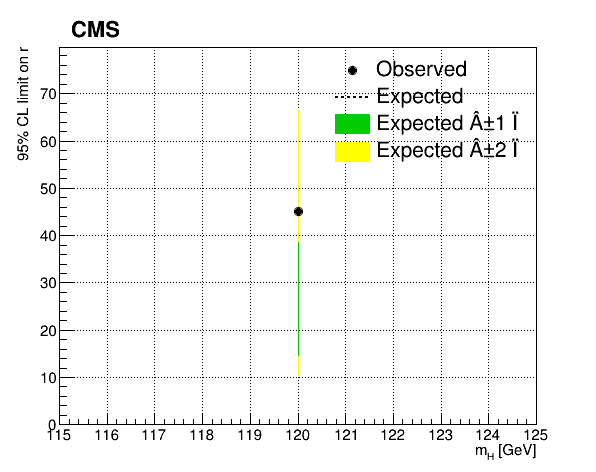
\includegraphics[keepaspectratio,alt={MuTau limits}]{datacards/MuTau_limits.png}}
\caption{MuTau limits}
\end{figure}
\end{frame}
